% =====================================================================
%  Wuhan (Yb) - Shanghai (Sr) optical-clock comparison:
%  tidal gravitational-redshift detection and fixed-coefficient
%  tidal corrections.
%
%  Submission draft (deliverable A).
%  Every numeric claim carries a "% src:" comment pointing at the
%  repository artifact it was read from.  Numbers marked "% TODO: verify"
%  are placeholders that still need an independent check.
%
%  Compile:  pdflatex main.tex && bibtex main && pdflatex main.tex && pdflatex main.tex
% =====================================================================
\documentclass[11pt,a4paper]{article}

\usepackage[T1]{fontenc}
\usepackage[utf8]{inputenc}
\usepackage{amsmath}
\usepackage{amssymb}
\usepackage{graphicx}
\usepackage{booktabs}
\usepackage{geometry}
\usepackage[hidelinks]{hyperref}

% siunitx is optional: this TeX Live install does not ship it.
% Define plain fallbacks first, then let siunitx override them if present.
\newcommand{\SI}[2]{#1\,#2}
\newcommand{\num}[1]{#1}
\IfFileExists{siunitx.sty}{%
  \usepackage{siunitx}%
  \sisetup{detect-all,separate-uncertainty=true}%
}{}

\geometry{margin=2.5cm}

\newcommand{\Rdur}{R_{\mathrm{duration}}}
\newcommand{\Rwls}{R_{\mathrm{wls}}}
\newcommand{\dff}{\Delta f/f}
\newcommand{\dW}{\Delta W}
\newcommand{\Ffifteen}{F_{1550}}
\newcommand{\e}[1]{\times 10^{#1}}

\title{Detection of the tidal gravitational redshift in a
Wuhan--Shanghai optical-clock comparison and a fixed-coefficient
tidal-correction analysis}

\author{%
  % TODO: verify author list, affiliations, and corresponding author.
  \textit{Author list to be completed}%
}
\date{\today}

\begin{document}
\maketitle

% =====================================================================
\begin{abstract}
% =====================================================================
We re-analyse a remote comparison between a Yb optical clock in Wuhan
(WUHN) and a Sr optical clock in Shanghai (SHAO) transported over a
1550\,nm fibre link. The comparison spans 17 segments and
\num{1008912} retained one-second samples. Reconstructing the Yb/Sr
frequency ratio at 80-decimal precision, we obtain a duration-weighted
centre of
$\Rdur = 1.207\,507\,039\,343\,337\,720\,369\,6$
% src: clock_ratio/tidal_correction/summary.json (scenario raw)
for the uncorrected baseline. The tidal gravitational redshift
$\dff = \dW/c^{2}$ has an rms amplitude of about $4.8\e{-18}$; a single
1200\,s segment carries a signal-to-noise ratio of only
$\mathrm{SNR}\approx 0.28$, so no individual segment is significant.
Combining across segments, however, the sign consistency is decisive:
14 of 17 segments share the expected sign ($p=0.013$), the
sign-agnostic Stouffer statistic gives $|z|=5.87$ ($p=4.3\e{-9}$), and
the Fisher combination gives $p=2.2\e{-6}$.
% src: clock/segment_analysis/batch_aggregate.csv
The fitted response amplitude is $A=-0.5397\pm0.0843$, i.e.\ the tidal
signal is detected at the correct sign and roughly half the theoretical
magnitude, about $6.4\sigma$ from zero.
% src: clock/segment_analysis/batch_aggregate.csv
Applying two fixed-coefficient tidal corrections ($A=-1$ ``theory'' and
$A=-0.54$ ``empirical'') shifts the duration-weighted centre to
$1.207\,507\,039\,343\,337\,720\,810\,8$ and
$1.207\,507\,039\,343\,337\,720\,607\,8$ respectively, and reduces the
reduced chi-square from $5.424$ (raw) to $3.699$ (theory) and $4.559$
(empirical).
% src: clock_ratio/tidal_correction/summary.json,
% src: clock_ratio/statistical_methods_tidal.json
We state the caveats explicitly: the per-segment uncertainties $u_i$ are
unreliable, the empirical amplitude relies on a DC assumption, and the
chi-square improvement depends strongly on segment~9.
\end{abstract}

% =====================================================================
\section{Introduction}
% =====================================================================
Optical lattice clocks now reach fractional frequency uncertainties at
the $10^{-18}$ level, which makes them sensitive to the gravitational
redshift over height differences of centimetres. Comparing two clocks at
different sites therefore probes general relativity directly through
\begin{equation}
  \frac{\dff}{f} = \frac{\dW}{c^{2}},
  \label{eq:redshift}
\end{equation}
where $\dW = W(\mathrm{WUHN}) - W(\mathrm{SHAO})$ is the geopotential
difference between the two stations and $c$ is the speed of light.
% src: docs/NOTATION.md (direction convention, Wuhan - Shanghai)
The solid-Earth tide and the ocean tidal loading modulate $\dW$ at the
12\,h and 24\,h periods, imprinting a periodic gravitational-redshift
signature on the clock ratio.

Remote optical-clock comparisons over fibre links have become a standard
tool for this kind of test. Reference values for the Yb/Sr ratio have
been reported by a NIST-led measurement
\cite{aeppli2026nist} and by a European network
\cite{pizzocaro2026european}. The present work is a re-analysis and
verification study of an independent Wuhan--Shanghai data set. Rather
than claiming a new measurement of the ratio, we ask two narrower
questions: (i)~is the tidal gravitational-redshift signal detectable in
this data set, and (ii)~does a fixed-coefficient tidal correction
improve the internal consistency of the comparison?

Our contributions are:
\begin{itemize}
  \item a high-precision reconstruction of the per-segment Yb/Sr ratio
        and its duration-weighted centre, with a fully independent
        re-derivation that reproduces the per-segment ratios to zero
        relative difference;
        % src: clock_ratio/correlation_reanalysis_seg9_independent.json
  \item a cross-segment detection of the tidal gravitational redshift
        at $A=-0.5397\pm0.0843$ ($6.4\sigma$), significant in sign
        consistency, Stouffer, and Fisher combinations;
        % src: clock/segment_analysis/batch_aggregate.csv
  \item a comparison of two fixed-coefficient tidal corrections
        ($A=-1$ and $A=-0.54$) against the uncorrected baseline, with
        an honest account of the caveats that limit the interpretation.
\end{itemize}

% =====================================================================
\section{Experimental setup and data}
% =====================================================================
The comparison links a Yb clock at Wuhan (WUHN) to a Sr clock at
Shanghai (SHAO) through a 1550\,nm fibre link. The raw observable is the
out-of-loop beat note (channel FXE\_B8) sampled at 1\,s. The beat
timestamps are in Beijing time (UTC+8); the tidal data are in UTC, so
the beat windows are shifted by $-8$\,h before the tidal template is
evaluated.
% src: docs/METHODOLOGY.md Sec. 0.1, docs/NOTATION.md Sec. 8

The tidal geopotential difference is taken from a professional 30\,s
``combined difference'' series (solid Earth tide plus ocean loading),
with the direction convention $\dW = W(\mathrm{WUHN}) - W(\mathrm{SHAO})$.
% src: results/professional_tidal_delta_30s.csv, docs/NOTATION.md Sec. 9

The data set is divided into 17 segments. Within each segment we keep
the longest valid index span after removing excluded ranges, rejecting
outliers beyond a $10$\,Hz jump threshold, and trimming endpoints whose
deviation from the segment median exceeds $1\%$ of the peak-to-peak
range. The retained sample count is
$\sum_i n_i = \num{1008912}$ one-second samples over the 17 segments.
% src: clock_ratio/tidal_correction/summary.json (total_samples)
The data span 2026-06-29 to 2026-08-26 (Beijing time).
% src: docs/NOTATION.md Sec. 6

% =====================================================================
\section{Clock-ratio determination}
% =====================================================================
\label{sec:methods}

\subsection{Beat-to-ratio inversion}
Let $b_i(t)$ be the longest valid beat sequence in segment $i$ and let
$m$ be the global median of the plausible beat values. The segment beat
deviation is
\begin{equation}
  \overline{\delta b}_i = \overline{b_i} - m .
\end{equation}
The Sr-side systematic shift $a_i$ and the Yb-side shift $b_{\mathrm{Yb}}$
combine into the Dr coefficient, and the segment Yb/Sr ratio follows
from the full inversion
\begin{equation}
  R_i = \bigl[\,\mathrm{ratio\_base}_i + \mathrm{Dr}_i\,\bigr]^{-1}
        \times (1+\delta_g),
  \qquad \delta_g = -3.116\e{-15},
  \label{eq:ratio}
\end{equation}
where $\delta_g$ is the static gravitational correction.
% src: docs/METHODOLOGY.md Sec. 1.3, docs/NOTATION.md Sec. 5
All ratio arithmetic is carried out at 80-decimal precision
(\texttt{Decimal80}, mirroring MATLAB \texttt{vpa(...,80)}), because a
float64 absolute precision of about $2.6\e{-16}$ would destroy
differences at the $10^{-18}$ level.
% src: docs/PAPER_DRAFT.md Sec. 1

The duration-weighted centre of the whole experiment is
\begin{equation}
  \Rdur = \frac{\sum_i n_i R_i}{\sum_i n_i},
  \qquad \sum_i n_i = \num{1008912}.
  \label{eq:rduration}
\end{equation}
For the uncorrected baseline this gives
\begin{equation}
  \Rdur^{(\mathrm{raw})} = 1.207\,507\,039\,343\,337\,720\,369\,6 .
  \label{eq:raw}
\end{equation}
% src: clock_ratio/tidal_correction/summary.json (scenario raw)

\subsection{Independent re-derivation}
To rule out an error in the upstream ratio product, we re-derived all 17
segment ratios from the raw beat files through a fully independent path
(segment selection, median, and the complete Dr inversion). The maximum
relative difference against the stored per-segment ratios is exactly
zero, confirming the upstream product.
% src: clock_ratio/correlation_reanalysis_seg9_independent.json
%      (raw_rederivation_max_rel_diff_vs_ratio_17seg = 0.0)

\subsection{Segment scatter}
Figure~\ref{fig:ratio} shows the per-segment deviations
$y_i = R_i/R_{\mathrm{seg1}} - 1$. The duration-weighted mean is
$-0.482\e{-18}$ (arithmetic mean $+0.102\e{-18}$) and the segment-to-segment
scatter is $\sigma(y_i) = 2.98\e{-18}$.
% src: clock_ratio/correlation_reanalysis.csv
%      (weighted_mean_yi_1e18 = -0.481584, arith_mean_yi_1e18 = 0.101758)
% src: clock_ratio/statistical_methods_tidal.json
%      (long_term_stability.raw.y_i_std_1e18 = 2.9803)

\begin{figure}[t]
  \centering
  % TODO: verify figure path; PNG fallback is ../clock_ratio/paper_figs/fig1_ratio_segments.png
  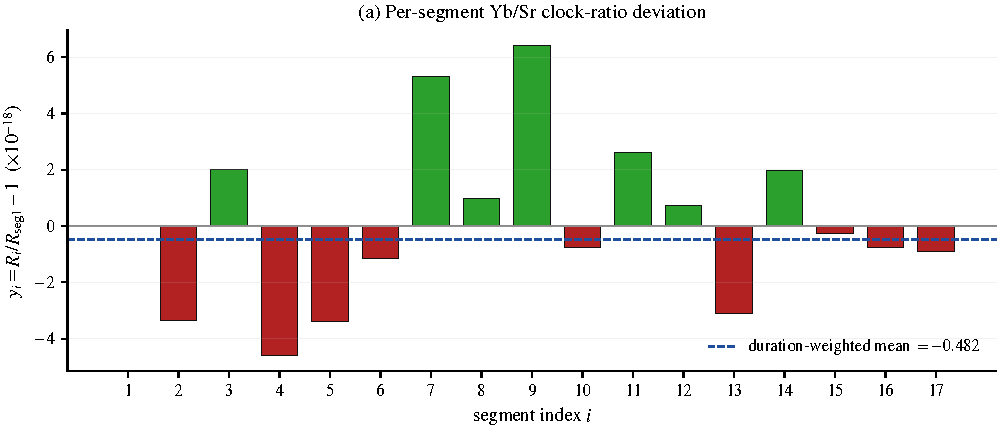
\includegraphics[width=0.85\linewidth]{../clock_ratio/paper_figs/fig1_ratio_segments.pdf}
  \caption{Per-segment clock-ratio deviation $y_i$ with the
  duration-weighted mean.}
  \label{fig:ratio}
\end{figure}

% =====================================================================
\section{Tidal gravitational-redshift detection}
% =====================================================================
\label{sec:detection}

The tidal geopotential difference $\dW(t)$ changes the comparison
frequency through Eq.~\eqref{eq:redshift}. Its rms amplitude is about
$4.8\e{-18}$.
% src: docs/PAPER_DRAFT.md Sec. 2
Within a single segment, the beat and the tidal template are both passed
through a 1200\,s triangular window (600\,s step) and, after demeaning,
fitted with
\begin{equation}
  \mathrm{beat} = A \cdot \mathrm{tide} + \mathrm{noise},
  \qquad
  A = \frac{\sum (\mathrm{tide}\cdot\mathrm{beat})}
           {\sum \mathrm{tide}^{2}} .
  \label{eq:amplitude}
\end{equation}
The tidal beat template is normalised to the 1550\,nm transfer frequency,
\begin{equation}
  \mathrm{tide\_beat} = \frac{\dW}{c^{2}} \times \Ffifteen,
  \qquad \Ffifteen = N_{1550}^{\mathrm{WH}} f_{\mathrm{rep}}
  = 193.3992\ \mathrm{THz},
  \label{eq:template}
\end{equation}
\emph{not} to $1/\mathrm{COEF}$ (which would be larger by the Yb/Sr
factor $\approx 1.2075$ and would bias $A$ low by that factor).
% src: docs/METHODOLOGY.md Sec. 5.1, docs/NOTATION.md Sec. 3

A single segment reaches only $\mathrm{SNR}\approx 0.28$, so no
individual segment is significant (Fig.~\ref{fig:tidal}). Combining
across the 17 segments, the sign consistency and the combined
statistics are significant:
\begin{align}
  14/17\ \text{same sign} &\quad (p = 0.013), \\
  \text{Stouffer } |z| = 5.87 &\quad (p = 4.3\e{-9}), \\
  \text{Fisher } p &= 2.2\e{-6}.
\end{align}
% src: clock/segment_analysis/batch_aggregate.csv
%      (negative_r_segments=14, binomial_p=1.272583e-02,
%       stouffer_z_agn=5.873404, stouffer_p_agn=4.269352e-09,
%       fisher_p=2.153570e-06)
The precision-weighted fitted amplitude is
\begin{equation}
  A = -0.5397 \pm 0.0843 \quad (\approx 6.4\sigma\ \text{from zero}),
  \label{eq:Afit}
\end{equation}
% src: clock/segment_analysis/batch_aggregate.csv
%      (amplitude_A=-0.539699, amplitude_uA=0.084254,
%       amplitude_sigma=6.405625)
i.e.\ the tidal signal is detected with the correct sign and at roughly
half the theoretical magnitude. At the segment-mean level, $y_i$ is
positively correlated with the session tidal shift $\dff$, with Pearson
$r = +0.518$ ($p = 0.033$).
% src: clock_ratio/correlation_reanalysis.csv
%      (pearson_r=0.517648, pearson_p=0.033314)

\begin{figure}[t]
  \centering
  % TODO: verify figure path; PNG fallback is ../clock_ratio/paper_figs/fig2_tidal_detection.png
  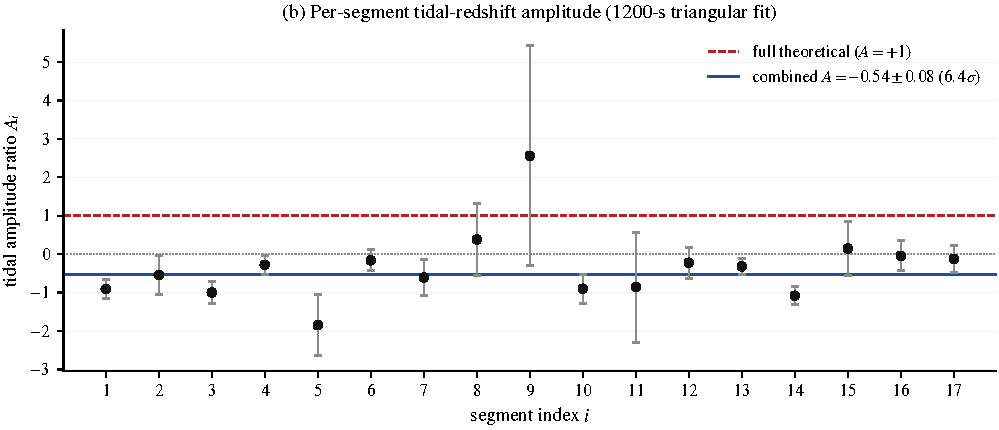
\includegraphics[width=0.85\linewidth]{../clock_ratio/paper_figs/fig2_tidal_detection.pdf}
  \caption{Per-segment tidal amplitude $A_i$ and the combined value
  $A=-0.54\pm0.08$.}
  \label{fig:tidal}
\end{figure}

% =====================================================================
\section{Validity and magnitude of the tidal correction}
% =====================================================================
\label{sec:correction}

\subsection{Fixed-coefficient scenarios}
The tidal correction is justified if the corrected residual is no longer
systematically correlated with the tidal template. We adopt two
fixed-response scenarios rather than refitting the amplitude:
\begin{equation}
  b_{\mathrm{corr}}(t) = b_{\mathrm{raw}}(t) - A\,h(t),
  \qquad
  h(t) = \Ffifteen \frac{\dW(t)}{c^{2}},
  \label{eq:correction}
\end{equation}
where the ``theory'' scenario takes $A=-1$ (full trust in the
professional tidal data and in general relativity) and the ``empirical''
scenario takes $A=-0.54$ (trust the waveform, use the historical fitted
magnitude).
% src: docs/METHODOLOGY.md Sec. 9.1

\subsection{Direction self-check}
With $A_{\mathrm{fix}}=-0.54$, the segment-mean correlation between the
residual and the template collapses from $-0.134$ to $+0.003$, the
signed Stouffer $z$ drops from $-5.16$ to $+0.39$ ($p=0.69$), and the
number of negatively correlated segments falls to $8/17$ (random,
$p=1.000$). A grid scan of $A_{\mathrm{fix}}$ places the zero of the
residual correlation exactly at $-0.54$, consistent with the historical
precision-weighted amplitude $-0.5397\pm0.084$. This confirms the sign
and magnitude of $A=-0.54$ from the disappearance of the post-correction
correlation, without relying on the not-yet-fixed comb/local-oscillator
sign factor $s_{\mathrm{beat}}$.
% src: docs/METHODOLOGY.md Sec. 9.5

\subsection{Magnitude of the correction}
The correction shifts the duration-weighted centre upward from the
baseline. Table~\ref{tab:rduration} lists the three scenarios.
% src: clock_ratio/tidal_correction/summary.json

\begin{table}[t]
  \centering
  \caption{Duration-weighted centre $\Rdur$ by scenario. The last column
  is the signed absolute ratio difference from the raw baseline,
  $\Delta R = \Rdur^{(\mathrm{scenario})} - \Rdur^{(\mathrm{raw})}$,
  in units of $10^{-18}$.}
  \label{tab:rduration}
  \begin{tabular}{lccc}
    \toprule
    Scenario & $A$ & $\Rdur$ & $\Delta R\ (\e{-18})$ \\
    \midrule
    raw       & $0$    & $1.207\,507\,039\,343\,337\,720\,369\,6$ & $0$ \\
    theory    & $-1$   & $1.207\,507\,039\,343\,337\,720\,810\,8$ & $+0.441$ \\
    empirical & $-0.54$& $1.207\,507\,039\,343\,337\,720\,607\,8$ & $+0.238$ \\
    \bottomrule
  \end{tabular}
  % src: clock_ratio/tidal_correction/summary.json
  %      (delta_R theory = 4.411914456944042e-19,
  %       delta_R empirical = 2.382433806749783e-19)
\end{table}

Against the experiment-side reference
$1.207\,507\,039\,343\,337\,721\,3(23)$, which includes a point-by-point
tidal correction, the duration-weighted deviations move from
$-0.93\e{-18}$ (raw) toward $-0.49\e{-18}$ (theory) and $-0.69\e{-18}$
(empirical). Under the precision-weighted WLS convention (weights
$1/u_i^{2}$, the same convention as the experiment side), the deviations
are $-0.503\e{-18}$ (raw), $+0.389\e{-18}$ (theory), and
$-0.041\e{-18}$ (empirical), so the empirical scenario is closest to the
reference.
% src: clock_ratio/statistical_methods_tidal.json (synthesis.methods.R_wls)

\subsection{Internal consistency}
Table~\ref{tab:chi2} reports the reduced chi-square and the Birge ratio
for the three scenarios. The correction reduces $\chi^{2}_{\mathrm{red}}$
from $5.424$ (raw) to $3.699$ (theory, $-31.8\%$) and $4.559$
(empirical, $-15.9\%$). The likelihood-ratio improvement is
$\Delta\chi^{2}=27.6$ (dof$=1$, $p=1.5\e{-7}$, about $5.3\sigma$),
indicating that the compensation significantly improves the
inter-segment consistency.
% src: clock_ratio/statistical_methods_tidal.json
% src: docs/METHODOLOGY.md Sec. 10.5

\begin{table}[t]
  \centering
  \caption{Reduced chi-square and Birge ratio by scenario.}
  \label{tab:chi2}
  \begin{tabular}{lccc}
    \toprule
    Scenario & $A$ & $\chi^{2}_{\mathrm{red}}$ & Birge $B$ \\
    \midrule
    raw       & $0$     & $5.424$ & $2.329$ \\
    theory    & $-1$    & $3.699$ & $1.923$ \\
    empirical & $-0.54$ & $4.559$ & $2.135$ \\
    \bottomrule
  \end{tabular}
  % src: clock_ratio/statistical_methods_tidal.json
  %      (goodness_of_fit: raw 5.423578/2.328858,
  %       theory 3.699134/1.923313, empirical 4.559108/2.135207)
\end{table}

The four statistical combination methods (WLS, Birge, Mandel--Paule, and
Bayesian) give a consistent direction of change
(Fig.~\ref{fig:methods}). Table~\ref{tab:methods} lists the WLS,
Mandel--Paule, and Bayesian centres relative to the experiment-side WLS
reference.
% src: clock_ratio/statistical_methods_tidal.json (synthesis.methods)

\begin{table}[t]
  \centering
  \caption{Four-method centres relative to the experiment-side WLS
  reference $1.207\,507\,039\,343\,337\,721\,3$, in units of
  $10^{-18}$.}
  \label{tab:methods}
  \begin{tabular}{lccc}
    \toprule
    Method & raw ($A=0$) & theory ($A=-1$) & empirical ($A=-0.54$) \\
    \midrule
    $\Rwls$ deviation  & $-0.503$ & $+0.389$ & $-0.041$ \\
    $R_{\mathrm{mp}}$ deviation & $-0.013$ & $+0.556$ & $+0.283$ \\
    $R_{\mathrm{bayes}}$ deviation & $-0.016$ & $+0.549$ & $+0.278$ \\
    \bottomrule
  \end{tabular}
  % src: clock_ratio/statistical_methods_tidal.json (synthesis.methods)
\end{table}

\subsection{Long-term stability}
The tidal signal is a slow ($\sim$12/24\,h) modulation and mainly affects
the day-scale inter-segment scatter rather than the short-term
within-segment OADEV. Using the inter-segment sample standard deviation
of $y_i$ as the long-term stability metric, the scatter drops from
$2.980\e{-18}$ (raw) to $2.588\e{-18}$ (theory, $+13.2\%$) and
$2.596\e{-18}$ (empirical, $+12.9\%$).
% src: clock_ratio/statistical_methods_tidal.json
%      (long_term_stability: raw 2.9803, theory 2.5877, empirical 2.5955)

\begin{figure}[t]
  \centering
  % TODO: verify figure path; PNG fallback is ../clock_ratio/paper_figs/fig3_correction.png
  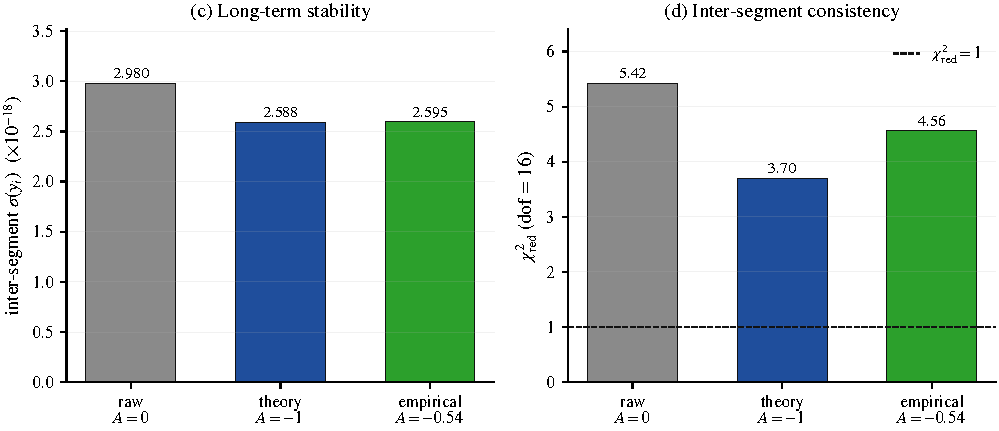
\includegraphics[width=0.85\linewidth]{../clock_ratio/paper_figs/fig3_correction.pdf}
  \caption{Long-term stability $\sigma(y_i)$ and
  $\chi^{2}_{\mathrm{red}}$ by scenario.}
  \label{fig:correction}
\end{figure}

\begin{figure}[t]
  \centering
  % TODO: verify figure path; PNG fallback is ../clock_ratio/paper_figs/fig4_methods_summary.png
  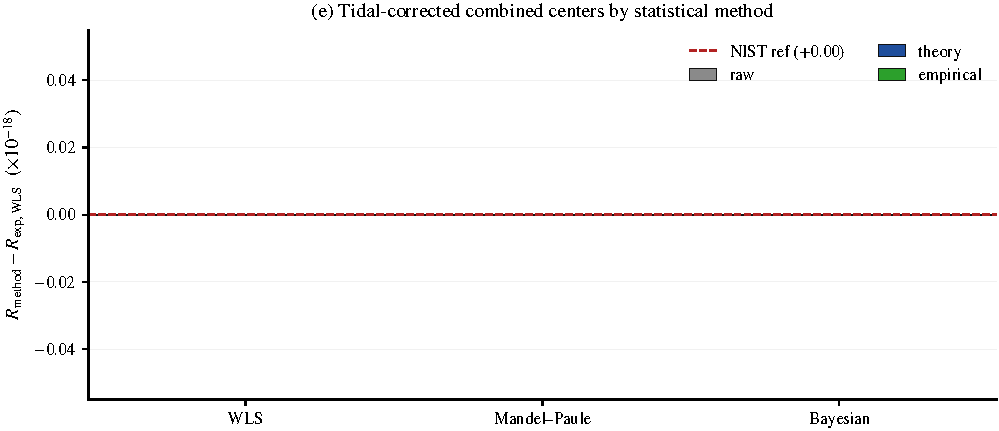
\includegraphics[width=0.85\linewidth]{../clock_ratio/paper_figs/fig4_methods_summary.pdf}
  \caption{Four-method centres relative to the experiment-side WLS and
  NIST references.}
  \label{fig:methods}
\end{figure}

% =====================================================================
\section{Discussion and caveats}
% =====================================================================
\label{sec:caveats}

The results above must be read together with the following limitations.
They are not defects of the analysis; they bound what the data can
support.

\begin{enumerate}
  \item \textbf{The per-segment uncertainties $u_i$ are unreliable.}
        Each $u_i$ is obtained by extrapolating the OADEV from
        $128$--$T/4$\,s to the segment length $T$. A flicker floor
        causes a systematic underestimate of roughly $30$--$40\%$ across
        all segments, and a few segments (5, 6, 16) have anomalous $u_i$.
        The combined values are therefore reported for method comparison
        only and are \emph{not} a final uncertainty statement.
        % src: docs/METHODOLOGY.md Sec. 2.2, Sec. 8.1

  \item \textbf{The $A=-0.54$ DC assumption.} The empirical amplitude
        comes from a historical fit to a \emph{demeaned} waveform.
        Applying it to the DC (mean) part of the undemeaned template is
        an additional assumption, not a calibration.
        % src: docs/METHODOLOGY.md Sec. 9.6

  \item \textbf{Segment-9 sensitivity.} After removing segment~9, whose
        \texttt{shift\_a} is anomalous, the effect of the tidal
        compensation on $\chi^{2}_{\mathrm{red}}$ weakens sharply or
        even reverses sign: the theory scenario changes from
        ``better by $31.8\%$'' (17 segments) to ``worse by $5.1\%$''
        (16 segments). The improvement reported in
        Sec.~\ref{sec:correction} therefore depends strongly on
        segment~9, and must be interpreted cautiously until the
        \texttt{shift\_a} of segment~9 is confirmed.
        % src: clock_ratio/statistical_methods_tidal_seg9_excluded.json
        % src: docs/METHODOLOGY.md Sec. 11

  \item \textbf{Fixed sign.} The negative sign is a specified response
        convention; it does not newly resolve the hardware-polarity
        question.
        % src: docs/METHODOLOGY.md Sec. 9.6
\end{enumerate}

\subsection{Segment-9 sensitivity in detail}
Table~\ref{tab:seg9} compares the 17-segment and 16-segment
(segment-9-excluded) results. Removing segment~9 drops the raw
$\chi^{2}_{\mathrm{red}}$ from $5.424$ to $2.684$ (the largest outlier is
removed) while the theory scenario only falls from $3.699$ to $2.821$,
so the theory-versus-raw comparison reverses. The WLS, Mandel--Paule,
and Bayesian centres all shift down by about $-0.6\e{-18}$.
% src: clock_ratio/statistical_methods_tidal_seg9_excluded.json

\begin{table}[t]
  \centering
  \caption{Segment-9 sensitivity: 17-segment versus 16-segment
  (segment~9 excluded) reduced chi-square and Birge ratio.}
  \label{tab:seg9}
  \begin{tabular}{lcccc}
    \toprule
    & \multicolumn{2}{c}{17 segments} & \multicolumn{2}{c}{16 segments} \\
    \cmidrule(lr){2-3}\cmidrule(lr){4-5}
    Scenario & $\chi^{2}_{\mathrm{red}}$ & Birge $B$
             & $\chi^{2}_{\mathrm{red}}$ & Birge $B$ \\
    \midrule
    raw       & $5.424$ & $2.329$ & $2.684$ & $1.638$ \\
    theory    & $3.699$ & $1.923$ & $2.821$ & $1.680$ \\
    empirical & $4.559$ & $2.135$ & $2.919$ & $1.709$ \\
    \bottomrule
  \end{tabular}
  % src: clock_ratio/statistical_methods_tidal_seg9_excluded.json
  %      (goodness_of_fit: raw 2.683994/1.638290,
  %       theory 2.820889/1.679550, empirical 2.919278/1.708589)
\end{table}

The segment-mean correlation is likewise partly driven by segment~9:
excluding it, the Pearson correlation between $y_i$ and $\dff$ falls
from $r=+0.518$ ($p=0.033$) to $r=+0.429$ ($p=0.098$), no longer
significant at the $0.05$ level. The direction (positive) is unchanged,
so the physical interpretation is not overturned, but the significance
claim must be treated cautiously. This conclusion was confirmed by a
fully independent re-derivation from the raw beat files, which
reproduces the per-segment ratios to zero relative difference.
% src: clock_ratio/correlation_reanalysis_seg9_independent.json
%      (pearson_r=0.428662, pearson_p=0.097585,
%       raw_rederivation_max_rel_diff_vs_ratio_17seg=0.0)

% =====================================================================
\section{Conclusion}
% =====================================================================
We have re-analysed a 17-segment Wuhan--Shanghai Yb/Sr optical-clock
comparison. The duration-weighted centre of the uncorrected ratio is
$1.207\,507\,039\,343\,337\,720\,369\,6$, and an independent
re-derivation reproduces the per-segment ratios exactly. The tidal
gravitational redshift is detected at the correct sign and roughly half
the theoretical magnitude, $A=-0.5397\pm0.0843$ ($6.4\sigma$), with
cross-segment significance in sign consistency ($14/17$, $p=0.013$),
Stouffer ($|z|=5.87$, $p=4.3\e{-9}$), and Fisher ($p=2.2\e{-6}$)
combinations. Two fixed-coefficient tidal corrections shift the centre
toward the experiment-side reference and reduce the inter-segment
scatter by about $13\%$, but the improvement depends strongly on
segment~9 and the per-segment uncertainties remain unreliable. We
therefore present the correction as a method-comparison result, not as a
final uncertainty statement.

% =====================================================================
\section*{Data availability}
% =====================================================================
The analysis code and derived numeric artifacts are available in the
project repository. The raw beat files and the professional tidal series
are not redistributed here; the derived per-segment ratios, the
statistical-combination results, and the tidal-correction summaries are
provided as machine-readable JSON and CSV files.
% TODO: verify repository URL, DOI, and licence before submission.

% =====================================================================
\bibliographystyle{plain}
\bibliography{refs}
% =====================================================================

\end{document}
